%! alt A regular 12-gon inscribed in its circumcircle with centre O. Points X and Y on the circumcircle lie in the gaps on either side of a run of four consecutive vertices, and M is the midpoint of the arc XY through the run. Two circles pass through X and Y with their centres on ray OM: the nearer one, drawn solid, encloses the run and O, and the farther one, drawn dashed, encloses the run but not O. Neither encloses any other vertex.
%! after_paragraph 2
%! scale 3/2
% The shared preamble of every Cevian figure. pipeline/figures turns these colours into theme-aware paint,
% and refuses any other colour, so draw only with them:
%   figink (lines and labels), figaux (construction lines), figaccent (the object the argument turns on),
%   figtint and figaccenttint (light fills).
\documentclass[border=1.5pt]{standalone}
\usepackage{tkz-euclide}
\definecolor{figink}{RGB}{0,0,0}
\definecolor{figaux}{RGB}{85,85,85}
\definecolor{figaccent}{RGB}{192,57,43}
\definecolor{figtint}{RGB}{221,221,221}
\definecolor{figaccenttint}{RGB}{245,213,208}
% tkz-euclide's defaults draw circles, compasses and marks in 50% grey and fill points with a tint.
\makeatletter
\def\tkz@otherlinecolor{figink}
\def\tkz@euc@circlecolor{figink}
\def\tkz@euc@compasscolor{figink}
\def\tkz@euc@mkcolor{figink}
\def\tkz@mk@fill{figink}
\def\tkz@euc@pointfillcolor{figink}
\makeatother
\tkzSetUpLine[color=figink,line width=.7pt]
\tkzSetUpArc[color=figink,line width=.7pt]
\tkzSetUpCompass[color=figink,line width=.5pt]
\tkzSetUpPoint[color=figink,fill=figink,size=3.1pt]
\tikzset{
  every picture/.style={line cap=round,line join=round,color=figink},
  circle style/.append style={color=figink,line width=.7pt},
  aux/.style={color=figaux,line width=.45pt,dash pattern=on 2.6pt off 2pt},
  key/.style={color=figaccent,line width=1pt},
  mk/.style={color=figink,line width=.5pt},
  lbl/.style={color=figink,inner sep=2.2pt},
  len/.style={color=figink,inner sep=1.5pt,font=\small},
}

\begin{document}
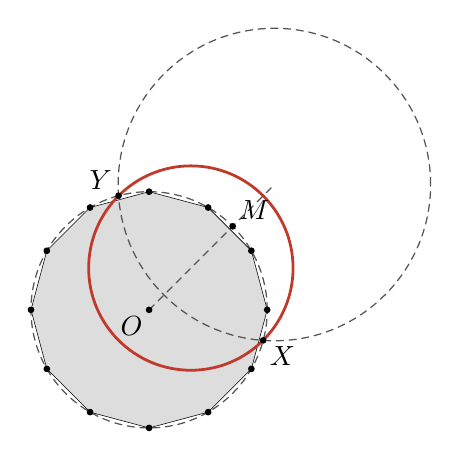
\begin{tikzpicture}
\tkzDefPoint(0.0,0.0){O} %! O = (0, 0)
\tkzDefPoint(1.5000000,0.0){V0} %! V0 = polar(O, 1, 0)
\tkzDefPoint(1.2990381,0.75000000){V1} %! V1 = polar(O, 1, 30)
\tkzDefPoint(0.75000000,1.2990381){V2} %! V2 = polar(O, 1, 60)
\tkzDefPoint(0.0000000000000000000000000000000000000000000000000032511253,1.5000000){V3} %! V3 = polar(O, 1, 90)
\tkzDefPoint(-0.75000000,1.2990381){V4} %! V4 = polar(O, 1, 120)
\tkzDefPoint(-1.2990381,0.75000000){V5} %! V5 = polar(O, 1, 150)
\tkzDefPoint(-1.5000000,0.0000000000000000000000000000000000000000000000000065022505){V6} %! V6 = polar(O, 1, 180)
\tkzDefPoint(-1.2990381,-0.75000000){V7} %! V7 = polar(O, 1, 210)
\tkzDefPoint(-0.75000000,-1.2990381){V8} %! V8 = polar(O, 1, 240)
\tkzDefPoint(-0.0000000000000000000000000000000000000000000000000097533758,-1.5000000){V9} %! V9 = polar(O, 1, 270)
\tkzDefPoint(0.75000000,-1.2990381){V10} %! V10 = polar(O, 1, 300)
\tkzDefPoint(1.2990381,-0.75000000){V11} %! V11 = polar(O, 1, 330)
\tkzDefPoint(1.4488887,-0.38822857){X} %! X = polar(O, 1, -15)
\tkzDefPoint(-0.38822857,1.4488887){Y} %! Y = polar(O, 1, 105)
\tkzDefPoint(1.0606602,1.0606602){M} %! M = polar(O, 1, 45)
\tkzDefPoint(0.53033009,0.53033009){Ka} %! Ka = polar(O, 1/2, 45)
\tkzDefPoint(1.5909903,1.5909903){Kb} %! Kb = polar(O, 3/2, 45)
%! fact collinear(Ka, O, M)
%! fact collinear(Kb, O, M)
%! fact equal(dist(Ka, X), dist(Ka, Y))
%! fact equal(dist(Kb, X), dist(Kb, Y))
%! fact dist(Ka, O) < dist(Ka, X)
%! fact dist(Kb, O) > dist(Kb, X)
%! fact dist(Ka, V0) < dist(Ka, X)
%! fact dist(Ka, V3) < dist(Ka, X)
%! fact dist(Ka, V4) > dist(Ka, X)
%! fact dist(Ka, V11) > dist(Ka, X)
%! fact dist(Kb, V0) < dist(Kb, X)
%! fact dist(Kb, V3) < dist(Kb, X)
%! fact dist(Kb, V4) > dist(Kb, X)
%! fact dist(Kb, V11) > dist(Kb, X)
%! example angle(X, O, Y) == 120
\tkzDrawCircle[aux](O,V0)
\tkzFillPolygon[color=figtint](V0,V1,V2,V3,V4,V5,V6,V7,V8,V9,V10,V11)
\tkzDrawPolygon(V0,V1,V2,V3,V4,V5,V6,V7,V8,V9,V10,V11)
\tkzDrawCircle[key](Ka,X)
\tkzDrawCircle[aux](Kb,X)
\tkzDrawSegment[aux](O,Kb)
\tkzDrawPoints(O,V0,V1,V2,V3,V4,V5,V6,V7,V8,V9,V10,V11,X,Y,M)
\tkzLabelPoint[below left,lbl](O){$O$}
\tkzLabelPoint[below right,lbl](X){$X$}
\tkzLabelPoint[above left,lbl](Y){$Y$}
\tkzLabelPoint[above right,lbl](M){$M$}
\end{tikzpicture}
\end{document}
